\chapter{Die Realisierung}
\label{cha:Realisierung}
Folgendes Kapitel befasst sich mit der Implementierung, der im Kapitel \ref{cha:Lösungskonzept} vorgestellten Spezifikation des Vorlagenmanagements. Die Implementierung wurde in \emph{Java 8} mit dem \emph{Buildtool Maven} realisiert, wobei die Implementierungen in der folgenden Projektstruktur organisiert wurden.
\begin{figure}[h]
\dirtree{%
.1 mailing.
.2 model.
.3 jpa.
.2 module.
.3 template.
.4 cdi.
.4 jsf.
.4 model.
.5 json.
.4 logic.
.5 api.
.5 impl.
.3 integration.
.4 clevercure-web.
.2 testsuite.
.3 cdi.
.2 demo.
.3 logic.
.3 web.
.2 data.
.3 api.
.3 impl.
}
\caption{Verzeichnisstruktur der \emph{Maven}-Projekte}
\label{fig:minimal-example:frame-dirtree}
\end{figure}
\ \newline
Das \emph{Maven} Wurzelprojekt \emph{mailing} organisiert alle Abhängigkeiten für die Unterprojekte, sowie die auf alle Unterprojekte anwendbare \emph{Build}-Konfiguration. Das Wurzelprojekt \emph{mailing} definiert auch die Metadaten, wie die EntwicklerInnen, die an diesem Projekt mitwirken. Dar Wurzelprojekt \emph{mailing} ist vom Typ \emph{pom}, was bedeutet, dass aus diesem Projekt kein Artefakt erstellt werden kann und es existiert um tiefer liegende Projekte zu bündeln. Projekte unterhalb von \emph{mailing}, die ebenfalls als \emph{pom} definiert wurden, sind aus der Sicht ihrer Kinder das Wurzelprojekt und könnten für diese Projekte Abhängigkeiten, oder \emph{Build}-Konfigurationen organisieren. Die gesamte Organisation der Abhängigkeiten findet im Wurzelprojekt \emph{mailing} statt. Diese Projektstruktur wurde gewählt, da in diesem Projekt auch die Implementierungen der anderen Softwarekomponenten des \emph{Mail-Service} organisiert werden. Die konkreten Artefakte wurden jeweils in ein Artefakt \emph{*-api} und \emph{*-impl} aufgeteilt, somit sind die Schnittstellen (Spezifikation) vollständig getrennt von deren Implementierungen. Folgende Auflistung beschreibt alle konkreten Artefakte (Java)-Archiv, die aus dem Projekt \emph{mailing} erstellt werden können.
\begin{itemize}
	\item\emph{\textbf{mailing-model-jpa}} 
	\newline
	ist das Artefakt, das die \emph{JPA 2.1 (JSR 338)} Klassen enthält, die die Datenbank in \emph{Java} abbilden.
	\item\emph{\textbf{mailing-module-template-cdi}} 
	\newline
	ist das Artefakt, das die Implementierung für die Integration in eine \emph{CDI 1.1 (JSR 346)} Umgebung  enthält.
	\item\emph{\textbf{mailing-module-template-jsf}}
	\newline
	ist das Artefakt, das die Implementierung für die Integration in \emph{JSF 2.2 (JSR 344)} enthält.
	\item\emph{\textbf{mailing-module-template-model-json}}
	\newline
	ist das Artefakt, das die Implementierung der \emph{JSON}-Spezifikation in Form von \emph{Java}-Klassen enthält.	
	\item\emph{\textbf{mailing-module-template-logic-api}} 
	\newline
	ist das Artefakt, das die Spezifikation des Vorlagenmanagement enthält.
	\item\emph{\textbf{mailing-module-template-logic-impl}} 
	\newline
	ist das Artefakt, das die Implementierung der Spezifikation des Vorlagenmanagements enthält.
	\item\emph{\textbf{mailing-module-integartion-clevercure-web}}
	\newline
	ist das Artefakt, das die Implementierung der Integration für die Anwendung \emph{CleverWeb} enthält.
	\item\emph{\textbf{mailing-testsuite-cdi}},
	\newline
	ist das Artefakt, das die Ressourcen aller Tests, die in einer \emph{CDI}-Umgebung lauffähig sein müssen, bereitgestellt.
	\item\emph{\textbf{mailing-demo-logic}}
	\newline
	ist das Artefakt, das den \emph{Service}-Schicht der Beispielanwendung darstellt.
	\item\emph{\textbf{mailing-demo-web}}
	\newline
	ist das Artefakt, das die Demowebanwendung darstellt.
	\item\emph{\textbf{mailing-data-api}}
	\newline
	ist das Artefakt, dass die Spezifikation der \emph{Services} enthält, die die Persistenz der \emph{E-Mail} behandeln. Es enthält auch die Datenbankzugriffsklassen in Form von \emph{Data-Repository}-Schnittstellen.
	\item\emph{\textbf{mailing-data-impl}}
	\newline
	ist das Artefakt, das die Implementierung der \emph{Service}-Spezifikation enthält.
\end{itemize} 

\section{Die Implementierung der Spezifikationen}
Der folgende Abschnitt behandelt die Implementierungen der im Kapitel \ref{cha:Lösungskonzept} vorgestellten Spezifikation. Es werden alle Implementierung der Spezifikationen bezüglich des Vorlagenmanagements behandelt und nicht für die Spezifikationen für die Persistenz, des Datenmodels und der Datenzugriffsschicht. Die nicht behandelten Softwarekomponenten wurden im Zuge der Entwicklung des Vorlagenmanagements, implementiert und stellen bereits einen Teil der Implementierung des \emph{Mail-Service} dar.

\subsection{Die Implementierung für \emph{CKEditor}}
\emph{Editor CKEditor} ist ein \emph{Javascript} basierter \emph{Editor}, mit dem die Vorlagen bearbeitet werden können. Er stellt Funktionalitäten wie z.B. Schriftarten und Schriftformen
zur Verfügung, was das Erstellen einer Vorlage auf Basis von \emph{HTML} erleichtert. Wie im Abschnitt \ref{sec:sub-typescript-javascript} vorgegeben, wird ein \emph{Plugin} benötigt, dass innerhalb des \emph{CKEDitors} die Variablen verwalten kann. Diese \emph{Plugin} wurde in \emph{Typescript} implementiert, mit dem im Gegenzug zu Javascript Typsicherheit gewährleistet werden kann. Die Implementierung des \emph{Plugins} in \emph{Typescript} war möglich, da für den \emph{CKEditor} vom dem \emph{Open-Source} Projekt \emph{DefinitelyTyped} Typinformationen für \emph{Typescript} bereitgestellt werden, die die \emph{Javascript}-Schnittstellen als \emph{Typescript}-Schnittstellen definieren, damit in \emph{Typescript} die Typsicherheit gewährleistet werden kann. Würden keine Typinformationen zur Verfügung stehen, hätte man sie selber implementieren müssen, was einen erheblichen Mehraufwand bedeutet hätte.
 
\subsubsection{Das \emph{CKEDitor-Plugin} in \emph{Typescript}}
Da das Variablenmanagement unabhängig vom verwendeten \emph{CKEditor} sein soll, wurde die Verwaltung der Variablen von dem \emph{CKEditor-Plugin} logisch und physisch getrennt, wobei das Variablenmanagement im \emph{Typescript}-Modul \emph{cc.variables} und das \emph{CKEDitor-Plugin} im \emph{Typescript}-Modul \emph{cc.ckeditor.plugins} organisiert wurden. Beide \emph{Typescript}-Quelltexte wurden in ihren eigenen Quelltextdateien implementiert und werden beim Kompilieren in eine einzige \emph{Javascript} zusammengeführt. Mit der Organisation in eigenen \emph{Typescript}-Modulen wird sichergestellt, dass nur explizit nach außen sichtbar gemachte \emph{(export MyType \{...\})} Funktionen oder Typen außerhalb des Moduls zur Verfügung stehen. Das \emph{Typescript}-Modul wird in ein korrespondierendes \emph{Javascript}-Modul übersetzt. Die folgenden Abbildungen \ref{prog:example-typescript-modul} und \ref{prog:example-javascript-modul} zeigen ein \emph{Typescipt}-Modul und das daraus resultierende \emph{Javascript}-Modul.
\begin{program}[h]
\caption{Das \emph{Typescript}-Modul}
\label{prog:example-typescript-modul}
\begin{JsCode}[numbers=none]
module cc.ckeditor.plugins {
	export module variables {
		export interface VariableMapping{
	        id:string
		}
	}
}                  
\end{JsCode}
\end{program}
\begin{program}[h]
\caption{Das resultierende \emph{Javascript}-Modul}
\label{prog:example-javascript-modul}
\begin{JsCode}[numbers=none]
var cc;
(function (cc) {
    var variables;
    (function (variables_1) {
    // VariableMapping is not present in javascript
    })(variables = cc.variables || (cc.variables = {}));
})(cc || (cc = {}));                 
\end{JsCode}
\end{program}
\ \newline
Die \emph{Typescript}-Schnittstelle \emph{VariableMapping} aus Quelltext \ref{prog:example-typescript-modul} ist nicht Teil des resultierenden \emph{Javascript}-Moduls, da diese Schnittstelle nur eine Typinformation für \emph{Typescript} darstellt und daher nicht Teil des resultierenden \emph{Javascript} ist. Wäre die Schnittstelle \emph{VariableMapping} eine \emph{Typescript}-Klasse, dann wäre sie auch Teil des resultierenden \emph{Javascripts} und würde als \emph{Javascript}-Funktion abgebildet werden.
\newline
\newline
Das Variablenmanagement in \emph{Typescript} ist verantwortlich für die \emph{Browser} seitige Registrierung der Variablen und stellt Hilfsmethoden zur Verfügung, mit denen Variablen gefunden und konvertiert werden können. Der Quelltext aus \ref{prog:example-typescript-convert-variable} zeigt wie eine Variable in \emph{Typescript} konvertiert werden kann.
\newpage
\begin{program}[h]
\caption{\emph{Typescript}-Funktion für die Variablenkonvertierung}
\label{prog:example-typescript-convert-variable}
\begin{JsCode}[numbers=none]
// Signature of the converter function
public convertVariables(converter:(item:VariableMapping) => any 
                        = (item:VariableMapping)=> item):any[]

// Convert to the variable's set displayName
variablesHandler.convertVariables(
	function (variable) {
		return variable.displayName;
	}
)                        
\end{JsCode} 
\end{program}
\ \newline
Die Funktion \emph{convertVariables} aus dem Quelltext \ref{prog:example-typescript-convert-variable} definiert den Formalparameter \emph{converter} als eine sogenannte \emph{Arrow}-Funktion, die einer \emph{Lambda}-Funktion in \emph{Java} ähnelt. Mit der \emph{Arrow}-Funktion wird die Signatur der Funktion für die Konvertierung definiert. In dem Quelltext aus \ref{prog:example-typescript-convert-variable} wird für den Formalparameter \emph{converter} eine Standardimplementierung bereitgestellt, die verwendet wird, sollte bei der Aktivierung der Funktion \emph{convertVariables} für den Formalparameter \emph{converter} kein Aktualparameter bereitgestellt werden. Der Typ \emph{any[]} ist vergleichbar mit dem Datentyp \emph{var} aus \emph{.NET} und gibt an das jeder Datentyp als Typ des zurückgelieferten \emph{Arrays} erlaubt ist.
\newline
\newline
Das \emph{CKEditor-Plugin} ist für die Integration der Variablen in den \emph{Editor} verantwortlich, wobei die zur Verfügung stehenden Variablen über einen Dialog ausgewählt werden können. Ausgewählte Variablen werden an die aktuelle Position des Cursors im \emph{HTML}-Dokuments des \emph{Editors} in Form eines \emph{HTML-Tags} platziert. Die \emph{HTML}-Repräsentation der Variable ist gekoppelt an den \emph{FacesConverter}, da der Konverter die Variable von dessen \emph{HTML}-Repräsentation in die \emph{Template-Engine} spezifische Repräsentation der Variablen  konvertieren muss. Die verwendete \emph{Template-Engine} ist für dieses \emph{Plugin} und das \emph{Javascript} seitige Variablenmanagement irrelevant, da die Variablen im \emph{Javascript} seitigen Variablenmanagement immer in der gleichen Objektrepräsentation vorhanden sind und im \emph{CKEditor-Plugin} immer der gleichen \emph{HTML}-Repräsentation verwendet werden. Lediglich der \emph{FacesConverter} ist gekoppelt and die verwendete \emph{Template-Engine}.
\newline
\newline
Die Abbildung \ref{fig:ckeditor-toolbar-opne-dialog} zeigt die Funktionsleiste des \emph{CKEditors}, in die der rot markierte \emph{Button} eingefügt wurde, über den ein Dialog geöffnet werden kann, über den die Variablen ausgewählt werden können. Dieser Dialog enthält alle Variablen, die im \emph{Javascript} seitigen Variablenmanagement registriert wurden und somit dem \emph{CKEDitor-Plugin} zur Verfügung stehen.
\begin{figure}[h]
\centering
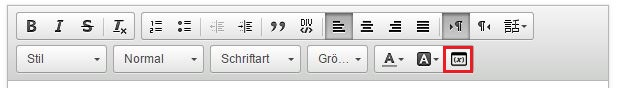
\includegraphics[scale=0.7]{ckeditor-toolbar-open-dialog}
\caption{\emph{CKEditor Toolbar Button} zum Öffnen des Dialogs}
\label{fig:ckeditor-toolbar-opne-dialog}
\end{figure}
\ \newline
Die Abbildung \ref{fig:ckeditor-dialog-insert-variable} zeigt den Dialog der vom \emph{CKEditor-Plugin} bereitgestellt wird. In diesem Dialog stehen alle registrierten Variablen zur Auswahl. Der Titel der Variable ist der Text in der Auswahlkomponente und die Beschreibung der ausgewählten Variable wird unterhalb der Auswahlkomponente angezeigt, wenn eine Variable ausgewählt wurde. Durch den Klick auf den \emph{Button OK} wird die Variable in die Vorlage eingefügt und der Dialog wird geschlossen.
\begin{figure}[h]
\centering
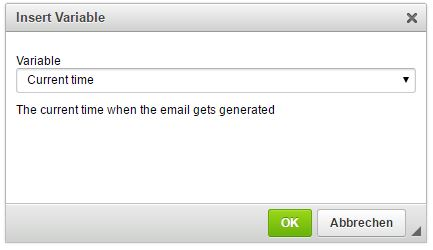
\includegraphics[scale=1]{ckeditor-dialog-insert-variable}
\caption{\emph{CKEditor} Dialog für die Variablenauswahl}
\label{fig:ckeditor-dialog-insert-variable}
\end{figure}
\ \newline
Die Abbildung \ref{fig:ckeditor-example-template} zeigt eine Vorlage innerhalb des \emph{CKEditors}, wobei die eingefügten Variablen besonders hervorgehoben werden. Der Titel der Variable stellt den Namen für den \emph{HTML-Tag} bereit und die Beschreibung dessen Titel. Die eingefügten \emph{HTML-Tags} dürfen nicht verändert werden, daher ist das \emph{Drag and Drop} und das Selektieren dieses eingefügten Texts nicht erlaubt, da dadurch die \emph{HTML}-Repräsentation der Variablen zerstört werden könnte und die Variablen nicht mehr vom \emph{FacesConverter} gefunden werden können.
\begin{figure}[h]
\centering
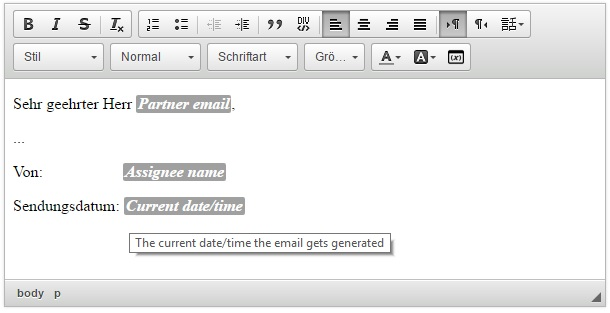
\includegraphics[scale=0.8]{ckeditor-example-template}
\caption{Beispiel einer Vorlage im \emph{CKEditor}}
\label{fig:ckeditor-example-template}
\end{figure}
\newpage

\subsubsection{Die Variablenrepräsentation in \emph{JSON}}
Die Variablen werden \emph{Java} seitig als Objekte der Schnittstelle \emph{VariableContract} abgebildet, und müssen für das \emph{Javascript} seitige Variablenmanagement in eine \emph{JSON}-Zeichenkette überführt werden, die als \emph{Javascript}-Objekt innerhalb des \emph{Javascript} seitige Variablenmanagements verwendet werden. Dafür wurde in \emph{Typescript} die Schnittstelle \emph{VariableMapping} aus dem Quelltext \ref{prog:example-typescript-variable-mapping} definiert, die die Struktur einer Variable innerhalb von \emph{Typescript} spezifiziert.
\begin{program}[h]
\caption{\emph{Typescript}-Funktion für die Variablenkonvertierung}
\label{prog:example-typescript-variable-mapping}
\begin{JsCode}[numbers=none]
interface VariableMapping {    
	id:string,       
	displayName:string,        
	info:string,
}
\end{JsCode}
\end{program}
\ \newline
Die Schnittstelle \emph{VariableMapping} ist Teil des Moduls \emph{cc.variables} und wird mit dem Schlüsselwort \emph{export} nach außen offengelegt und kann über den vollständigen Pfad \emph{cc.variables.VariableMapping} innerhalb von \emph{Typescript} verwendet werden. Mit der Schnittstelle \emph{VariableMapping} werden Typinformationen für der Variablenpräsentation in \emph{Typescript} bereitgestellt, damit innerhalb von \emph{Typescript} die Typsicherheit der Variablenrepräsentation sichergestellt werden kann.
\newline
\newline
Der Quelltext aus \ref{prog:variableJson} zeigt die korrespondierende Implementierung der \emph{JSON}-Spezifikation in \emph{Java} mit der Klasse \emph{VariableJson}. Mit der Klasse \emph{VariableJson} wird sichergestellt, das die Variablenrepräsentation in \emph{Java} korrespondierend zur Variablenrepräsentation in \emph{Typescript} ist. Als \emph{JSON-Provider} wird die Bibliothek \emph{fasterxml-jackson-json}, vormals \emph{jackson-json}, verwendet, die es erlaubt mit Annotationen deklarativ Attribute und/oder Methoden einer Klasse auf \emph{JSON}-Attribute abzubilden. Durch diesen deklarativen Ansatz sind die Attribute und/oder die Methoden einer Klasse entkoppelt von der \emph{JSON}-Spezifikation und können daher abgeändert werden. Nur ein Ändern des Datentyps eines Attributes kann zu Problemen führen. 
\begin{program}[h]
\caption{VariableJson.java}
\label{prog:variableJson}
\begin{JsCode}
@JsonTypeName(value = "variable-json")
public class VariableJson extends AbstractJsonModel {

    private String id;
    private String label;
    private String info;

    public VariableJson() {
    }

    public VariableJson(String id, String displayName, String tooltip) {
        this.id = id;
        this.label = displayName;
        this.info = tooltip;
    }

    @JsonGetter("id")
    public String getId() { return id; }

    @JsonSetter("id")
    public void setId(String id) { this.id = id; }

    @JsonGetter("displayName")
    public String getLabel() { return label; }

    @JsonSetter("displayName")
    public void setLabel(String label) { this.label = label; }

    @JsonGetter("info")
    public String getInfo() { return info; }

    @JsonSetter("info")
    public void setInfo(String info) { this.info = info; }
}
\end{JsCode}
\end{program}
\ \newpage

\subsection{Die Implementierungen für \emph{CDI}}
Folgender Abschnitt behandelt die Implementierungen für die Integration in eine \emph{CDI}-Umgebung. Wie in Abschnitt \ref{sec:sub-template-management-cdi} beschrieben, sollen die Variablen beim Start der Anwendung, die in einer \emph{CDI}-Umgebung läuft, automatisch  registriert werden. Das Vorlagenmanagement stellt Ressourcen die folgend aufgelisteten Ressourcen kontextabhängig über einen implementierten \emph{CDI}-Erzeuger zur Verfügung. 
\begin{itemize}
 \item Objekte der Schnittstelle \emph{VariableConfiguration} sind Objekte, die die registrierten Variablen verwalten.
 \item Objekte der Schnittstelle \emph{TemplateDataJsonBuilder} sind Objekte, mit denen das Datenobjekt in Form von \emph{JSON} für eine Vorlage und eine spezifische \emph{Template-Engine} erstellt werden kann.
 \item Objekte der Schnittstelle \emph{TemplateProcessor} sind Objekte, mit denen Variablen in Vorlagen verwaltet werden können.
 \item Objekte der Klasse \emph{CdiTemplateUtil} sind Objekte mit denen die registrierten Variablen, die Objekte der Schnittstelle \emph{VariableContract} sind, in Objekte der Klasse \emph{VariableJson} konvertieren kann, wobei der Titel und die Beschreibung sprachspezifisch gesetzt werden.
\end{itemize}

\subsubsection{Die Vorlagenmanagement \emph{CDI}-Erweiterung}
Um die Variablen beim Start der Anwendung innerhalb einer \emph{CDI}-Umgebung automatisch registrieren zu können, wurde eine \emph{CDI}-Erweiterung \emph{TemplateCdiExtension} implementiert, die das Variablenmanagement in eine \emph{CDI}-Umgebung integriert. Eine Erweiterung für eine \emph{CDI}-Erweiterung muss folgende Voraussetzungen erfüllen. 
\begin{enumerate}
	\item Die Schnittstelle \emph{javax.enterprise.inject.spi.Extension} implementieren und
	\item in einer Datei namens \emph{javax.enterprise.inject.spi.Extension}, die im Verzeichnis \emph{META-INF/services} liegen muss, mit ihren vollständigen Namen registriert werden.
\end{enumerate}
Durch die Datei \emph{javax.enterprise.inject.spi.Extension} wird die Erweiterung der \emph{CDI}-Umgebung bekannt gemacht und wird beim Start der \emph{CDI}-Umgebung geladen und kann auf Ereignisse des Lebenszyklus reagieren, in dem Sie Beobachtermethoden implementiert, die für die einzelnen Ereignisse aufgerufen werden. Die Schnittstelle \emph{javax.enterprise.inject.spi.Extension} ist ein Interface, das keine abstrakten Methoden enthält und als Markierung fungiert, um ein Klasse als \emph{CDI}-Erweiterung zu markieren. Die Erweiterung wird über den \emph{Service-Provider-Interface (SPI)} Mechanismus geladen.
\newline
\newline
Eine \emph{CDI}-Erweiterung ist an sich kein \emph{CDI-Bean}, da das Objekt der \emph{CDI}-Erweiterung bereits beim Start des \emph{CDI-Containers} erstellt wird und somit schon existiert bevor die \emph{CDI}-Umgebung vollständig gestartet wurde. Trotzdem ist das Objekt der \emph{CDI}-Erweiterung injizierbar und kann in \emph{CDI-Beans} injiziert werden. Das erstellte Objekt der \emph{CDI}-Erweiterung \emph{TemplateCdiExtension} existiert über die Lebensdauer der \emph{CDI}-Umgebung.
\newline
\newline
Der Quelltext aus Abbildung \ref{prog:templateCdiExtension} ist ein Auszug aus der implementierten \emph{CDI}-Erweiterung \emph{TemplateCdiExtension} und zeigt die Beobachtermethoden, die Lebenszyklus Ereignisse der \emph{CDI}-Umgebung beobachten. Über die \emph{CDI}-Erweiterung des Vorlagenmanagements werden alle implementierten Typen der Schnittstelle \emph{VariableContract} über die Beobachtermethoden gefunden und im Objekt der Klasse \emph{TemplateConfiguration} registriert, das über die Lebensdauer der \emph{CDI}-Erweiterung existiert. Es werden nur Implementierungen der Schnittstelle \emph{VariableContract} unterstützt, die als \emph{enum} implementiert wurden, obwohl auch Implementierung von Klassen unterstützt werden könnten, in dem die Typen der Schnittstelle \emph{VariableContract} gesammelt und im weiteren Programmverlauf  manuell aus der \emph{CDI}-Umgebung geholt werden könnten. Es werden auch alle implementierten Typen der Schnittstelle \emph{VariableResolverFactory} gefunden und in der \emph{CDI}-Erweiterung registriert.
\begin{program}[h]
\caption{Auszug aus der \emph{CDI}-Erweiterung \emph{TemplateCdiExtension}}
\label{prog:templateCdiExtension}
\begin{JavaCode}
public class TemplateCdiExtension implements Extension,
        Serializable {

    private TemplateConfiguration templateConfig;
    private Map<Class<? extends VariableContract>, 
                Class<VariableResolverFactory>>  
            variableResolverFactoryMap;

    void beforeBeanDiscovery(@Observes BeforeBeanDiscovery bbd) {
        // Init class members
    }

    <T> void processCdiVariableContracts
             (@Observes @WithAnnotations({BaseName.class, 
                                          CdiVariableContract.class}) 
             ProcessAnnotatedType<T> pat) {
       // Collect VariableContract types (Enum type only)
    }

    <T> void processVariableResolverFactoryFactories
        (@Observes @WithAnnotations(CdiVariableResolverFactory.class) 
        ProcessAnnotatedType<T> pat) {
        // Collect VariableResolverFactory types
    }
}
\end{JavaCode}
\end{program}
\ \newpage
\begin{itemize}
	\item\emph{void beforeBeanDiscovery(...)} 
	\newline
	ist die \emph{Observer}-Methode, die einmalig aufgerufen wird bevor mit dem Auffinden der \emph{CDI-Beans} begonnen wird. In dieser Methode wird die Extension initialisiert.
	\item\emph{<T> void processCdiVariableContracts(...)} 
	\newline
	ist die \emph{Observer}-Methode, die für jeden annotierten Typ aufgerufen wird, der mit den Annotationen \emph{@BaseName} und \emph{@CdiVariableContract} annotiert ist.
	\item\emph{<T> void processVariableResolverFactoryFactories(...)} 
	\newline
	ist die \emph{Observer}-Methode, die für jeden annotierten Typ aufgerufen wird, der mit den Annotationen \emph{@CdiVariableResolverFactory} annotiert ist.
\end{itemize}

\subsubsection{Der Vorlagenmanagement \emph{CDI}-Erzeuger}
Es wurde eine \emph{CDI}-Erzeuger Klasse \emph{TemplateResourceProducer} implementiert, mit der kontextabhängig Ressourcen des Vorlagenmanagements produziert werden. Diese Klasse ist die einzige Klasse, die sich die \emph{CDI}-Erweiterung \emph{TemplateCdiExtension} injizieren lässt. Es kann nicht verhindert werden, dass andere \emph{CDI-Beans} sich diese Klasse injizieren lassen, da eine \emph{CDI}-Erweiterung öffentlich sein muss. Es wir aber empfohlen, dass niemand außer die \emph{CDI}-Integration selbst sich das Objekt der \emph{CDI}-Erweiterung injizieren lässt.
\newline
\newline
Wie im Kapitel \ref{cha:Lösungskonzept} vorgegeben sollen mehrere \emph{Template-Engines} unterstützt werden, daher wurde die Annotation \emph{@FreemarkerTemplate} eingeführt, die einen Injektionspunkt für \emph{Freemarker} qualifiziert. In \emph{CDI} wird ein Qualifizierer benötigt, wenn für eine Schnittstelle bzw. eine Typ mehrere Implementierungen zur Verfügung stehen, da die \emph{CDI}-Umgebung in so einem Fall nicht entschieden kann welche Implementierung verwendet werden soll. Es wurde jeweils eine Erzeugermethode für den Qualifizierer \emph{@Default} und \emph{@FreemarkerTemplate} implementiert. Für den Qualifizierer \emph{@Default} wird die Implementierung für die \emph{Template-Engine Freemarker} verwendet, wodurch diese Implementierung als die Standardimplementierungen fungieren. Man setzt sich aber der Gefahr aus, dass die produzierte \emph{@Default} Implementierung nicht die gewollte ist. Der Qualifizierer muss an einem Injektionspunkt angegeben werden, wenn ein anderer Qualifizierer als \emph{@Default} verwendet werden soll. Der Qualifizierer \emph{@Default} wird immer als Standard Qualifizierer herangezogen, wenn keine expliziter Qualifizierer am Injektionspunkt angegeben wurde.
\newline
\newline
Der Quelltext aus Abbildung \ref{prog:templateResourceProducer} ist ein Auszug aus der Klasse \emph{TemplateResourceProducer} und zeigt einige der implementierten Erzeugermethoden. 
\newpage
\begin{program}[h]
\caption{TemplateResourceProducer.java}
\label{prog:templateResourceProducer}
\begin{JavaCode}
@ApplicationScoped
public class TemplateResourceProducer implements Serializable {
    @Produces
    @ApplicationScoped
    @Default
    public VariableConfiguration produceConfiguration() {
        return extension.getVariableConfiguration();
    }
    
    @Produces
    @Dependent
    @Default
    public TemplateDataJsonBuilder produceDefaultTemplateBuilder
          (final @Default VariableResolverFactoryProvider factory) {
        return produceFreeMarkerTemplateBuilder(factory);
    }

    @Produces
    @Dependent
    @FreemarkerTemplate
    public TemplateDataJsonBuilder produceFreeMarkerTemplateBuilder
           (final @Default VariableResolverFactoryProvider factory) {
        return new FreemarkerTemplateDataJsonBuilder()
                	.withWeakMode()
                	.withVariableResolverFactoryProvider(factory);
    }
}
\end{JavaCode}
\end{program}
\ \newline
Es wurden zwei Erzeugermethoden implementiert um Objekte der Schnittstelle \emph{TemplateDataJsonBuilder} zu erzeugen.
\begin{enumerate}
	\item\emph{produceDefaultTemplateBuilder} für \emph{@Default} Qualifizierer und 
	\item\emph{produceFreeMarkerTemplateBuilder} für \emph{@Freemarker} Qualifizierer.	
\end{enumerate}
\ \newline
Diese beiden Methoden produzieren Objekte für den sogenannten Pseudo-\emph{Scope @Dependent}, wobei für jeden Injektionspunkt ein neues Objekt erstellt wird. Der Lebenszyklus von \emph{CDI-Beans} im Pseudo-\emph{Scope @Default} wird nicht von der \emph{CDI}-Umgebung verwaltet. Beim Erzeugen eines solchen Objekts wird lediglich Injektion durchgeführt und die Lebensdauer eines solchen Objekts hängt davon ab, ob das Objekt noch referenziert wird. Als Argument für diesen beiden Methoden wird ein Objekt der Schnittstelle \emph{VariableResolverFactoryProvider} injiziert, das mit dem Qualifzierer \emph{@Default} annotiert ist. Dieses Objekt wird kontextabhängig injiziert, wobei der Geltungsbereich dieses Objekts für die Methoden nicht bekannt ist. 
\newline
\newline
Die Methode \emph{produceConfiguration} produziert ein Objekt der Schnittstelle  \emph{VariableConfiguration}, die die registrierten Variablen enthält und von der \emph{CDI}-Erweiterung bereitgestellt wird. Nachdem diese Schnittstelle nur lesenden Zugriff erlaubt und nur die \emph{CDI}-Erweiterung Variablen registriert, wird dieses Objekt für den Gültigkeitsbereich der Anwendung produziert, also einmalig für die gesamte Anwendungslaufzeit.

\subsubsection{Die Vorlagenmanagement \emph{CDI}-Hilfsklasse}
Die Klasse \emph{CdiTemplateUtil} wurde implementiert um ein injizierbares \emph{CDI-Bean} zur Verfügung zu stellen, das Hilfsmethoden für die Konvertierung der Variablen von Objekten der Schnittstelle \emph{VariableContract} in Objekte der Klasse \emph{VariableJson} und visa versa zur Verfügung stellt. Diese Implementierung ist statuslos, daher kann dieses \emph{CDI-Bean} in den Anwendungskontext gelegt werden.
\begin{program}[h]
\caption{CdiTemplateUtil.java}
\label{prog:cdiTemplateUtil}
\begin{JavaCode}
@ApplicationScoped
@Typed(CdiTemplateUtil.class)
public class CdiTemplateUtil implements Serializable {

    @Inject
    private VariableConfiguration config;

    public List<VariableJson> convertContractToJsonModel
    						  (final Locale locale) {
    }

    public List<VariableJson> convertContractToJsonModel
    		(final Collection<VariableContract> contracts,
             final Locale locale) {
    }

    public VariableJson convertContractToJsonModel
           (final VariableContract contract,
            final Locale locale) {
    }
	
    public List<VariableContract> convertJsonModelToContract
    							 (final Collection<VariableJson> jsonModels) {
    }

    public VariableContract convertJsonModelToContract
                            (final VariableJson jsonModel) {
    }
}
\end{JavaCode}
\end{program}
\newpage
\subsection{Die Implementierungen für \emph{JSF}}
Folgender Abschnitt behandelt die Implementierung des Variablenmanagements für die \emph{View}-Technologie \emph{JSF}. In diesem Abschnitt wird sich nur dem implementierten \emph{FacesConverter} und der \emph{CKEditor}-Integration, bereitgestellt von \emph{primefaces-extensions}, beschäftigen.

\subsubsection{Der Vorlagen \emph{FacesConverter}}
Es wurde der Konverter \emph{AbstractTemplateConverter} als abstrakte Klasse implementiert, die die Schnittstelle \emph{javax.faces.Converter} implementiert. Diese abstrakte Klasse wurde implementiert, da die Logik für die Konvertierung0 über alle \emph{Template-Engines} dieselbe ist und sich lediglich die Implementierung der Schnittstelle \emph{TemplateProcessor} unterschiedet. Das Objekt der Schnittstelle \emph{TemplateProcessor} und das Objekt der Klasse \emph{CdiTemplateUtil} werden manuell von der \emph{CDI}-Umgebung geholt, da keine Injektion innerhalb von \emph{JSF}-Artfakten in \emph{JSF 2.2} möglich ist. Die Injektion in \emph{JSF}-Artefakte wird erst ab \emph{JSF 2.3} unterstützt werden. Die Objekte werden über die Klasse \emph{BeanProvider} der Bibliothek \emph{Deltaspike} geholt, die Hilfsmethoden zur Verfügung stellt, mit denen man zur Laufzeit manuell mit der \emph{CDI}-Umgebung interagieren kann. \emph{Deltaspike} ist eine Bibliothek, die eine portable \emph{CDI}-Erweiterung darstellt. 
\newline
\newline
Die konkrete Implementierung \emph{FreemarkerTemplateConverter} für die \emph{Template-Engine Freemarker}, die von der abstrakten Klasse \emph{AbstractTemplateConverter} ableitet, setzt über einen Konstruktor in der Basisklasse den korrespondierenden Qualifizierer für die verwendete \emph{Template-Engine} und das zu verwendende Objekt der Klasse \emph{java.util.Locale}. Mit diesem Qualifizierer wird die korrekte Implementierung der Schnittstelle \emph{TemplateProcessor} aus dem \emph{CDI-Container} geholt. Da der Konverter eine Abhängigkeit auf ein \emph{Locale} Objekt besitzt, muss ein Objekt des Konverters im \emph{Quelltext} erzeugt und über Parameterbindung an eine \emph{JSF}-Komponente gebunden werden. Das Binden des Konverters an eine \emph{JSF}-Komponente über dessen Namen definierbar über die Annotation \emph{@FacesConverter("converterName")} ist nicht möglich. 
\newpage
\begin{program}[h]
\caption{FreemarkerTemplateConverter.java}
\label{prog:freemarkerTemplateConverter}
\begin{JavaCode}
public class FreemarkerTemplateConverter 
                          extends AbstractTemplateConverter {

    public FreemarkerTemplateConverter(final Locale locale) {
        super(new FreemarkerTemplateLiteral(), locale);
    }
}
\end{JavaCode}
\end{program}
\ \newline
Die abstrakte Klasse \emph{AbstractTemplateConverter} definiert reguläre Ausdrücke, um die Variablen einer Vorlage in Form von \emph{HTML-Tags} zu finden und zu konvertieren.
\begin{JavaCode}[numbers=none]
String tagRegex = "(<span[^,>]*class=\"variable\"[^,>]*>[^,<]*</span>)";
String idRegex = "data-variable-id=\"(\\S+)\"";
\end{JavaCode}
\ \begin{itemize}
	\item\emph{tagRegex} ist der reguläre Ausdruck, um die Variablen in ihrer \emph{HTML}-Repräsentation in einer Vorlage zu finden.
	\item\emph{idRegex} ist der reguläre Ausdruck, um die \emph{Id} einer Variable, aus deren \emph{HTML}-Repräsentation zu bekommen und wird auf den gefundenen \emph{HTML-Tag} einer Variable angewendet, die mit dem regulären Ausdruck \emph{tagRegex} gefunden wurde.
\end{itemize}
\ \newline
Die abstrakte Klasse \emph{AbstractTemplateConverter} definiert auch eine Vorlage in Form einer Zeichenkette, mit der die Variablen in ihre \emph{HTML-Tag}-Repräsentation konvertiert werden können, wobei diese Vorlage unabhängig von der verwendeten \emph{Template-Engine} ist und auf alle Variablen gleich angewendet werden kann.
\begin{JavaCode}
String template = "<span class=\"variable\" contentEditable=\"false\" "
                + "data-variable-id=\"{0}\" title=\"{1}\">{2}</span>";
\end{JavaCode}
Die Vorlage \emph{template} wird mit \emph{java.text.MessageFormat(String, Object...)} verarbeitet, wobei der Formalparameter \emph{Object...}, der eine variable Argumentliste repräsentiert, über den die dynamischen Werte für die Vorlage bereitgestellt werden können. 

\subsubsection{Die \emph{Primefaces-Extension} für den \emph{CKEditor}}
Der \emph{Rich-Editor CKEditor} ist eine \emph{Javascript} basierte Anwendung, die nur am \emph{Browser} der BenutzerInnen läuft. Es wird aber eine \emph{JSF}-Integration benötigt, damit man
\begin{itemize}
	\item auf \emph{AJAX-Events} reagieren kann,
	\item\emph{FacesConverter} verwenden kann und
	\item Parameterbindungen definieren kann.
\end{itemize}
\ \newline
Da es nicht trivial ist eine vollwertige \emph{JSF}-Komponente zu implementieren und das Implementieren einer solchen Komponente auch viel Zeit in Anspruch nimmt, wurde auf die Implementierung von \emph{Primefaces-Extensions} zurückgegriffen, die bereits eine vollwertige \emph{JSF}-Integration für den \emph{CKEditor} bereitstellt. \emph{Primefaces-Extensions} ist eine quelloffene Bibliothek, die die quelloffene Bibliothek \emph{Primefaces} erweitert. \emph{Primefaces} ist zurzeit eine der bekanntesten \emph{JSF}-Komponenten Bibliothek im \emph{Java}-Umfeld.
\newline
\newline
Die Ressourcen für den \emph{CKEDitor} bewegen sich in der Größenordnung von 1,5 Megabyte, daher werden die Ressourcen in einem separaten Artefakt zur Verfügung gestellt. Man kann auch eine eigene Implementierung zur Verfügung stellen, sofern diese Implementierung in derselben  Version vorhanden ist, wie von \emph{Primefaces-Extensions} unterstützt wird. Der \emph{CKEditor} ist ein sehr umfangreicher \emph{Editor}, den man sich auch seinen Wünschen entsprechend selbst zusammenstellen kann. Eine solche benutzerdefinierte Zusammenstellung des \emph{CKEditors} kann man heranziehen, um die Standardimplementierung zu ersetzen.
\newline
\newline
Der Quelltest aus Abbildung \ref{prog:example-ckeditor-xhtml} illustriert die Verwendung des \emph{CKEditors} in Form der zur Verfügung gestellten \emph{JSF}-Komponente.
\begin{program}[h]
\caption{\emph{XHTML-Markup} für \emph{CKEditor}}
\label{prog:example-ckeditor-xhtml}
\begin{HtmlCode}
<pe:ckEditor id="template_content_editor"
             wdgetVar="pfEditor"
             value="#{templateEditModel.content}"
             converter="#{ckeditorBean.converter}" 
             contentsCss="resources/css/myStyle.css"
             customConfig="./ckeditor-config.js">
</pe:ckEditor>
\end{HtmlCode}
\end{program}
\ \begin{itemize}
	\item\emph{id} ist das Attribute, um die eindeutige \emph{Id} innerhalb des Namensraums der Komponente zu definieren.
	\item\emph{widgetVar} ist das Attribut, um einen eindeutigen Name des \emph{Javascript}-Objekts, das den Zugriff auf den \emph{CKEditor} in \emph{Javascript} erlaubt, zu definieren.
	\item\emph{value} ist das Attribut, um die Parameterbindung der Vorlage zu einem \emph{Java}-Objekt zu definieren.
	\item\emph{converter} ist das Attribut, um den verwendeten Konverter, der die Vorlagen konvertiert, über Parameterbindung zu setzen.
	\item\emph{contentCss} ist das Attribut, um eine eigene \emph{CSS}-Datei für den Inhalt der Vorlage zu definieren. Die Vorlage wird innerhalb des \emph{Editors} als eigenständige \emph{HMTL}-Datei behandelt, das in einer \emph{Iframe}-Komponente gehalten wird.
	\item\emph{customConfig} ist das Attribut, um die eigene Konfiguration des \emph{Editors} in Form von einer eigenen \emph{Javascript}-Datei zu definieren. 
\end{itemize}

\section{Die Vorlagenmanagement Beispielanwendung}
Der folgende Abschnitt beschäftigt sich mit der implementierten Beispielanwendung, für das Vorlagenmanagement, die die Verwendung des Vorlagenmanagement im Bezug auf 
\begin{itemize}
	\item die Verwendung in der Geschäftslogik,
	\item die Verwendung über eine Webseite und
	\item die Verwendung zum Erstellen einer \emph{E-Mail}  
\end{itemize}
aufzeigen soll. Dazu wurde eine Demowebanwendung implementiert, die die Web seitige  Verwaltung der Vorlagen implementiert. Es wurde auch eine Klasse implementiert, die aufzeigen soll, wie eine \emph{E-Mail} basierend auf einer Vorlage, aus einer Geschäftslogik heraus erstellt werden kann. 

\subsection{Die Verwendung in einem \emph{Business}-Service}
Der folgende Quelltext aus Abbildung \ref{prog:emailServiceCdiEventImpl} zeigt wie eine \emph{E-Mail} über die die implementierte Klasse \emph{EmailServiceImpl} der Schnittstelle \emph{EmailService} erstellt werden kann. Das Objekt der Schnittstelle \emph{EmailService} wird über die \emph{CDI}-Umgebung zur Verfügung gestellt und mittels Injektion in die Geschäftslogik injiziert. Die Schnittstelle \emph{EmailService} und dessen Implementierung \emph{EmailServiceCdiEventImpl} befinden sich im Artefakt \emph{mailing-template-integration-clevercure-web}. Dieses Artefakt stellt die Integration in die Anwendung \emph{CleverWeb}  dar. Die \emph{E-Mails} werden in der Implementierung \emph{EmailServiceCdiEventImpl} über \emph{CDI-Events} erstellt, damit ist die Logik für das Erstellen der \emph{E-Mail} vollständig entkoppelt von dieser Implementierung. Im folgenden sind die zur Verfügung gestellten Methoden der Schnittstelle \emph{EmailService} angeführt, die der Geschäftslogik zur Verfügung stehen.
\begin{itemize}
	\item\emph{public void create(EmailDTO dto)}
	\newline
	ist die Methode, mit der eine \emph{E-Mail} sofort erstellt werden können.
	\item\emph{public void create(List<EmailDTO> dtos)}
	\newline
	ist die Methode, mit der mehrere \emph{E-Mails} sofort erstellt werden können.
	\item\emph{public void createAfterSuccess(EmailDTO dto)}
	\newline
	ist die Methode, mit der eine \emph{E-Mail} nach dem erfolgreichem Beenden einer Transaktion erstellt werden kann.
	\item\emph{public void createAfterSuccess(List<EmailDTO> dto)}
	\newline
	ist die Methode, mit der mehrere \emph{E-Mails} nach dem erfolgreichem Beenden einer Transaktion erstellt.
 werden kann.    
\end{itemize} 
\begin{program}[h]
\caption{EmailServiceCdiEventImpl.java}
\label{prog:emailServiceCdiEventImpl}
\begin{JavaCode}
@RequestScoped
@Transactional(Transactional.TxType.SUPPORTS)
public class EmailServiceCdiEventImpl implements EmailService {
    @Inject
    private Event<CreateEmailsEvent<CreateEmailsEvent.CreateImmediate>> createImmediateEvent;
    @Inject
    private Event<CreateEmailsEvent<CreateEmailsEvent.CreateAfterSuccess>> createAfterSuccessEvent;
    @Inject
    private Event<CreateEmailsEvent<CreateEmailsEvent.CreateAfter>> createAfterEvent;

    @Override
    @Transactional(Transactional.TxType.REQUIRED)
    public void create(EmailDTO dto) {
        createImmediateEvent.fire(new CreateEmailsEvent<>(dto));
    }

    @Override
    @Transactional(Transactional.TxType.REQUIRED)
    public void create(List<EmailDTO> dtos) {
        createImmediateEvent.fire(new CreateEmailsEvent<>(dtos));
    }

    @Override
    public void createAfterSuccess(EmailDTO dto) {
        createAfterSuccessEvent.fire(new CreateEmailsEvent<>(dto));
    }

    @Override
    public void createAfterSuccess(List<EmailDTO> dtos) {
        createAfterSuccessEvent.fire(new CreateEmailsEvent<>(dtos));
    }
}
\end{JavaCode}
\end{program}
\ \newline
Der Quelltext aus Abbildung \ref{prog:businessServiceImpl} zeigt das Beispiel der Geschäftslogik, die über die Schnittstelle \emph{EmailService} \emph{E-Mails} erstellt. Die zu erstellende \emph{E-Mail} wird durch ein Objekt der Klasse \emph{EmailDTO} repräsentiert, das alle benötigten Informationen für das Erstellen einer \emph{E-Mail} enthält.
\newpage
\begin{program}[h]
\caption{BusinessServiceImpl.java}
\label{prog:businessServiceImpl}
\begin{JavaCode}
@RequestScoped
@Transactional(Transactional.TxType.REQUIRED)
public class BusinessServiceImpl implements BusinesService {

    @Inject
    private EmailService emailService;

    @Override
    public void doBusinessEmailImmediate() {
        emailService.create(createEmailDto());
    }

    @Override
    public void doBusinessEmailAfterSuccess() {
        emailService.createAfterSuccess(createEmailDto());
    }

    private EmailDTO createEmailDto() {
        final String email = "herzog.thomas8@gmail.com";
        final Long mailUserId = 1L;
        final List<Long> mailTypeIds = Collections.singletonList(1L);
        final Locale locale = Locale.US;
        final ZoneId zone = ZoneId.systemDefault();
        final Map<Object, Object> userData = 
        	new HashMap<Object, Object>() {{
                put(TemplateVariable.SENDER_USER, "Thomas Herzog");
                put(TemplateVariable.RECIPIENT_USER, "Hugo Maier");
                put(TemplateVariable.TOPIC, "User status changed");
                put(TemplateVariable.STATUS, "Inactive");
            }};
        return new EmailDTO(email, 
        					locale, 
        					zone, 
        					mailUserId, 
        					userData, 
        					mailTypeIds);
    }
}
\end{JavaCode}
\end{program}
\ \newline
Folgende Auflistung erklärt die Attribute, die beim Erstellen eine Objekts der Klasse \emph{EmailDto} angegeben werden müssen.
\begin{itemize}
	\item\emph{email} ist die Zeichenkette, die die \emph{E-Mail}-Adresse definiert.
	\item\emph{mailUserId} ist die \emph{Id} des virtuellen Benutzers, der die \emph{E-Mail} auf der Datenbank erstellt.
	\item\emph{mailTypeIds} ist die Menge von \emph{Ids}, die die \emph{Mail}-Typen repräsentieren. Jedem \emph{Mail}-Typ ist eine Voralge zugeordnet.
	\item\emph{locale} ist das Objekt der Klasse \emph{java.util.Locale} , das die Sprache definiert.
	\item\emph{zone} ist das Objekt der Klasse \emph{java.time.ZoneId}, das die Zone für die Datumsformatierung definiert.
	\item\emph{userData} ist der assoziative Behälter, der die Benutzerdaten enthält, die bei der Evaluierung verwendet werden.
\end{itemize}

\subsection{Die Verwendung über eine \emph{Web}-Oberfläche}
Die Abbildung \ref{fig:demo_web_app_empty_view_part_1} zeigt die Weboberfläche, die für die Beispielanwendung implementiert wurde. Über dieses Formular können die Voralgen sprachspezifisch verwaltet werden.
\ \begin{figure}[h]
\centering
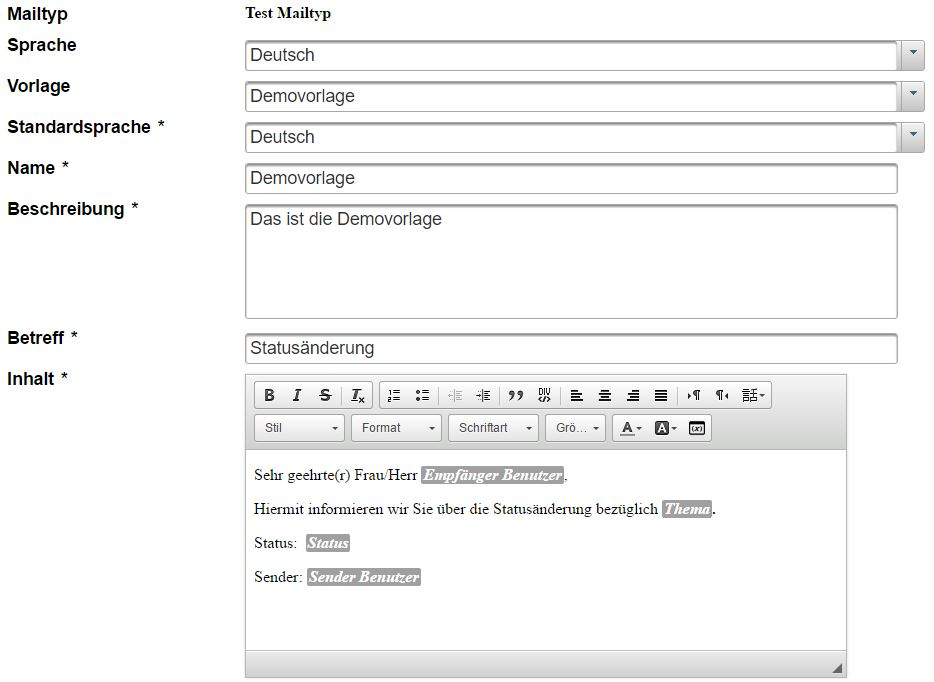
\includegraphics[scale=0.5]{demo_web_app_empty_view_part_1}
\caption{Formular für die Verwaltung der Vorlagen}
\label{fig:demo_web_app_empty_view_part_1}
\end{figure}
\ \newline
Die Abbildung \ref{fig:demo_web_app_empty_view_part_2} zeigt, den Teil der Webseite, der die relevanten Daten einer Vorlage anzeigt.
\begin{itemize}
	\item\emph{Decorator Template} ist die \emph{Freemarker}-Voralge, die von jeder Vorlage dekoriert wird.
	\item\emph{User Template} ist die Vorlage, die von einem BenutzerIn erstellt wurde.
	\item\emph{Template JSON Data} ist die \emph{JSON}-Zeichenkette, die erstellt wird, wenn die Daten für eine Vorlage serialisiert werden.
	\item\emph{Parsed Template} ist die Vorlage, in der die Variablen durch die serialisierten Werte ersetzt wurden.
	\item\emph{Template Metadata} sind die Metadaten der Vorlage, wie z.B. die Anzahl der enthalten Variablen.
\end{itemize}
\begin{figure}[h]
\centering
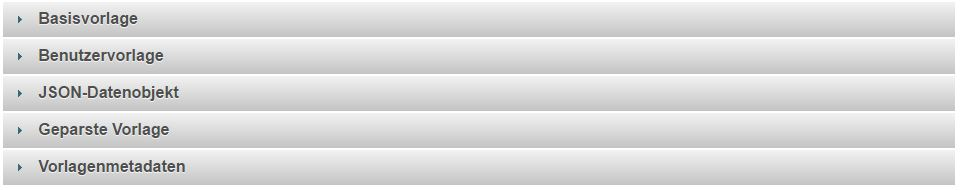
\includegraphics[scale=0.5]{demo_web_app_empty_view_part_2}
\caption{Anzeige der aller relevanten Daten einer Vorlage}
\label{fig:demo_web_app_empty_view_part_2}
\end{figure}

\subsubsection{Die dekorierbare Vorlage}
Die Abbildung \ref{fig:demo_web_app_data_decorator} zeigt die dekorierbare \emph{Freemarker}-Vorlage, die alle Vorlagen dekorieren. Sie stellt den \emph{HTML-Body} zur Verfügung, da die Benutzervoralgen nur den Inhalt innerhalb des \emph{HTML-Tags body} bereitstellen.
\begin{figure}[h]
\centering
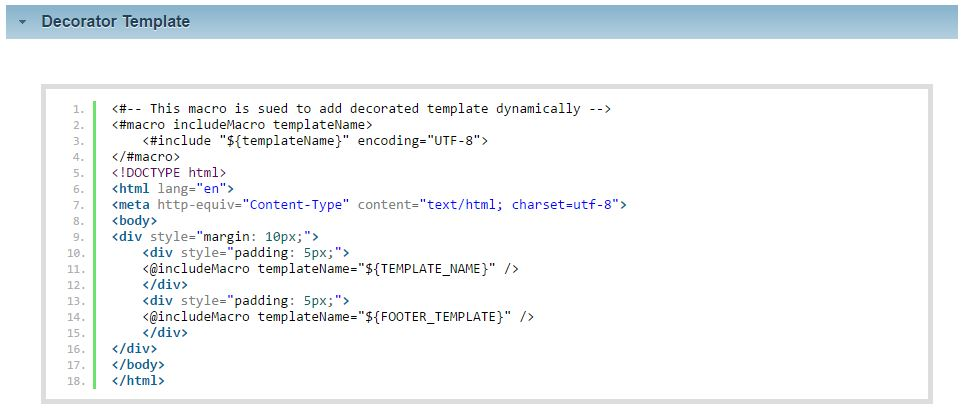
\includegraphics[scale=0.5]{demo_web_app_data_decorator}
\caption{Das \emph{Decorator Template}}
\label{fig:demo_web_app_data_decorator}
\end{figure}
\ \newpage

\subsubsection{Die Benutzervorlage}
Die Abbildung \ref{fig:demo_web_app_data_template} zeigt die \emph{Freemarker}-Vorlage, die von der BenutzerInnen erstellt wird. Die Vorlage enthält zwar \emph{HTML-Markup}, aber nur den Inhalt unterhalb des \emph{HTML-Tags body}. Sie stellt aber kein vollständiges \emph{HTML}-Dokument zur Verfügung.
\begin{figure}[h]
\centering
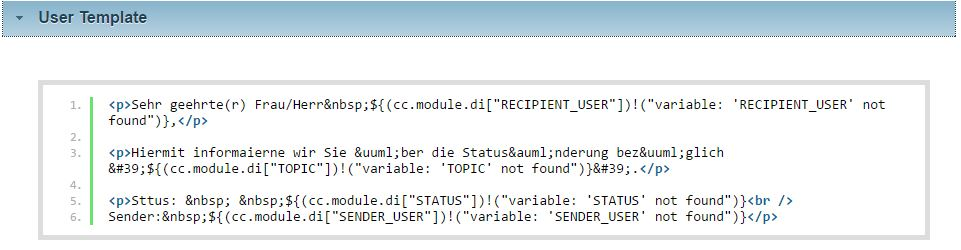
\includegraphics[scale=0.5]{demo_web_app_data_template}
\caption{Die \emph{Benutzervorlage} als \emph{Freemarker Template}}
\label{fig:demo_web_app_data_template}
\end{figure}

\subsubsection{Die serialisierte \emph{JSON}-Zeichenkette}
Die Abbildung \ref{fig:demo_web_app_data_json} zeigt die serialisierte \emph{JSON}-Zeichenkette, die beim Erstellen einer \emph{E-Mail} erstellt wird und in der Datenbank persistent gehalten wird. Mit diesen Daten kann eine \emph{E-Mail} auf Basis dieser Vorlage jederzeit wiederhergestellt werden.
\begin{figure}[h]
\centering
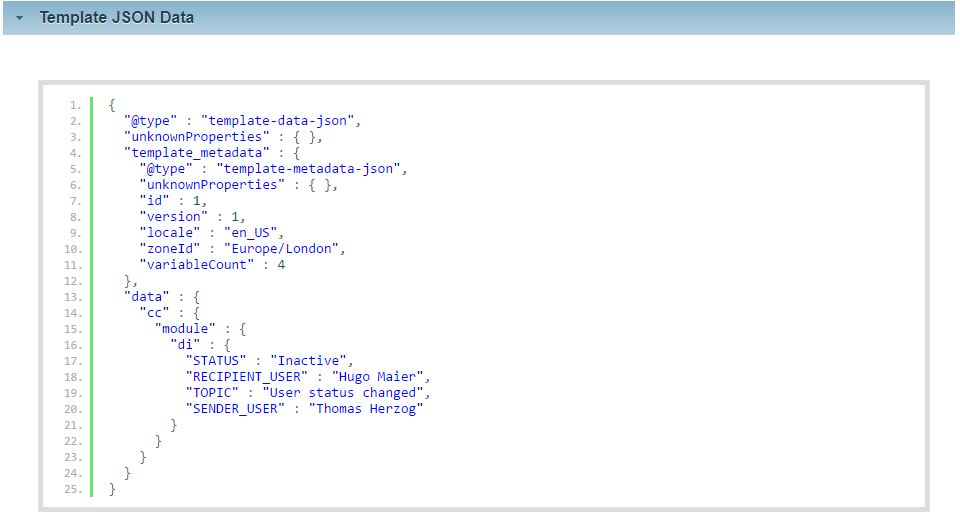
\includegraphics[scale=0.5]{demo_web_app_data_json}
\caption{Der serialisierte \emph{JSON}-String}
\label{fig:demo_web_app_data_json}
\end{figure}
\ \newpage

\subsubsection{Die Vorlagenmetadaten}
Die Abbildung \ref{fig:demo_web_app_data_metadata} zeigt die Metadaten der Benutzervorlage. Die Metadaten sind nur für die Entwicklung relevant.
\begin{figure}[h]
\centering
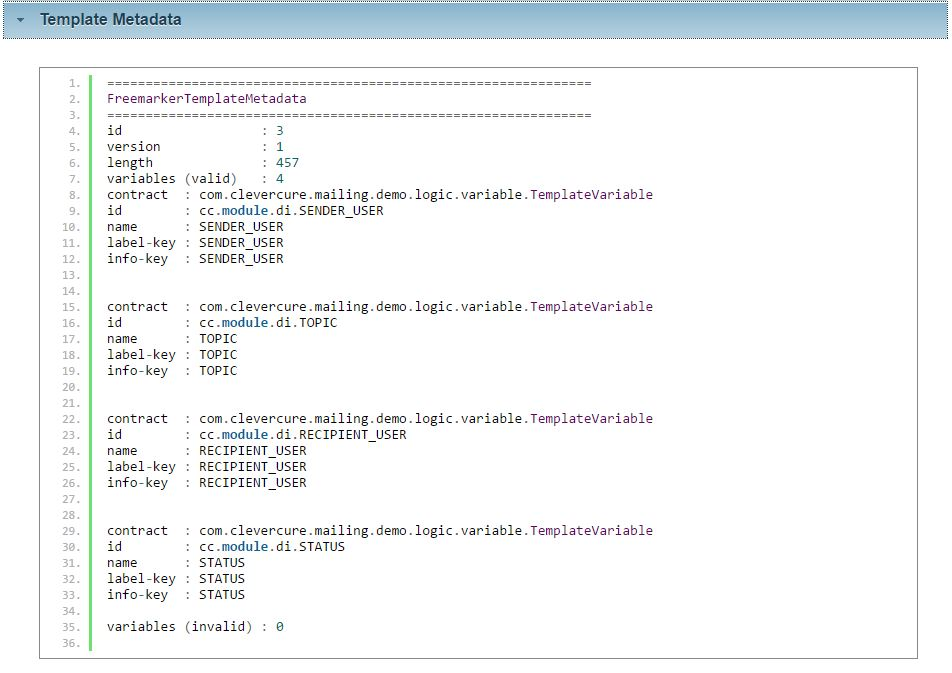
\includegraphics[scale=0.5]{demo_web_app_data_metadata}
\caption{Die Metadaten der Vorlage}
\label{fig:demo_web_app_data_metadata}
\end{figure}

\subsubsection{Der erstellte \emph{E-Mail}-Inhalt}
Die Vorlage mit den aufgelösten Variablen aus Abbildung \ref{fig:demo_web_app_data_parsed} zeigt die Metadaten der Benutzervorlage. 
\begin{figure}[h]
\centering
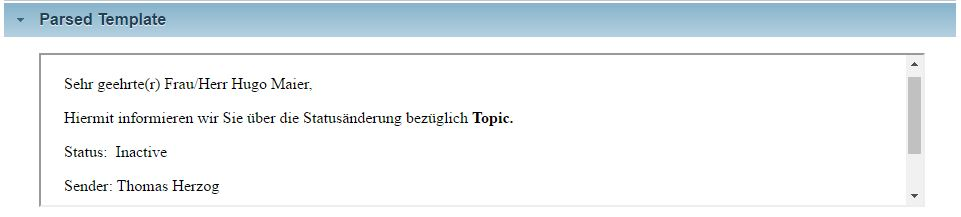
\includegraphics[scale=0.5]{demo_web_app_data_parsed}
\caption{Die Metadaten der Vorlage}
\label{fig:demo_web_app_data_parsed}
\end{figure}